\section{Supplementary experiments}\label{app:exp}
\subsection{Size convergence and mean reversal}\label{sec:convergence}
Figure~\ref{fig:convergence} shows the convergence diagnostics from the existing experiments. At $k=5$ and
$z_{\rm sh}\approx-3.5$, the conditional mean over all failure samples goes from about $+0.047$ at $M=256$ to
about $-0.473$ at $M=65536$. At the largest size, the prediction in shifted coordinates is about $-0.475$, and
the standard error of the simulated mean is about $0.015$. In other words, the negative offset at large size
matches the prediction; at small size the offset has the opposite sign, and this reversal disappears as $M$ grows.

The second panel shows the residuals of the macroscopic core conditional layer, referenced against the selection
law in empirical coordinates. Positive residuals appear at both values of $k$ and shrink as the size grows; this
is consistent with the roughly $M^{-1/2}$ contraction direction of the moderate deviation regime in
Appendix~\ref{app:exp-md}.
\begin{figure}[!htbp]
\centering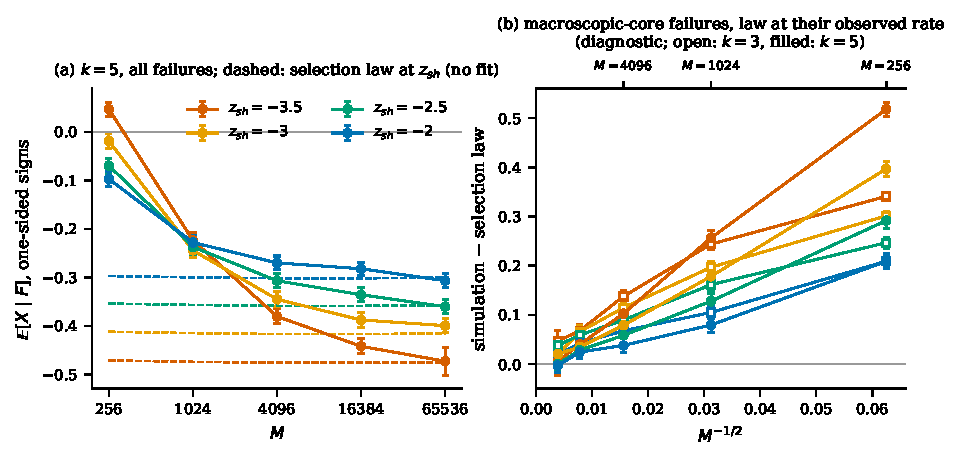
\includegraphics[width=\linewidth]{figures/fig_convergence.pdf}
\caption{Size convergence. (a) The conditional mean over all failure samples at $k=5$ and the analytic prediction of
the selection law; (b) residuals of the macroscopic core layer.}
\label{fig:convergence}
\end{figure}

\subsection{Range where the deep-left-tail approximation fails}
Figure~\ref{fig:leftrisk} shows the risk of the deep left tail. At $k=5$, $M=65536$, and $z_{\rm sh}\approx-3.5$, the
corrected nominal $1\%$ threshold produced 52 lower-tail observations among 4549 failure samples, an actual rate of
$1.14\%$, with a $95\%$ Wilson interval of $[0.87\%,1.50\%]$. The corresponding $k=3$ configuration gives 273 among
9021 failures, namely $3.03\%$, with interval $[2.69\%,3.40\%]$; if only the macroscopic core layer is considered,
the rate is about $0.71\%$.

This shows that at this finite size, small-core failures still affect the measurement distribution over all failure
samples. On the other hand, even when the macroscopic core dominates, calibration can still be off: at $k=5$ and
$M=256$ the deep-left-tail points are almost entirely macroscopic core failures, yet the actual rate of the nominal
$1\%$ threshold is only about $0.31\%$. The accuracy of the deep left tail is determined by two factors together: the
error of the conditional distribution itself at finite size, and the contamination from small-core failures.
\begin{figure}[!htbp]
\centering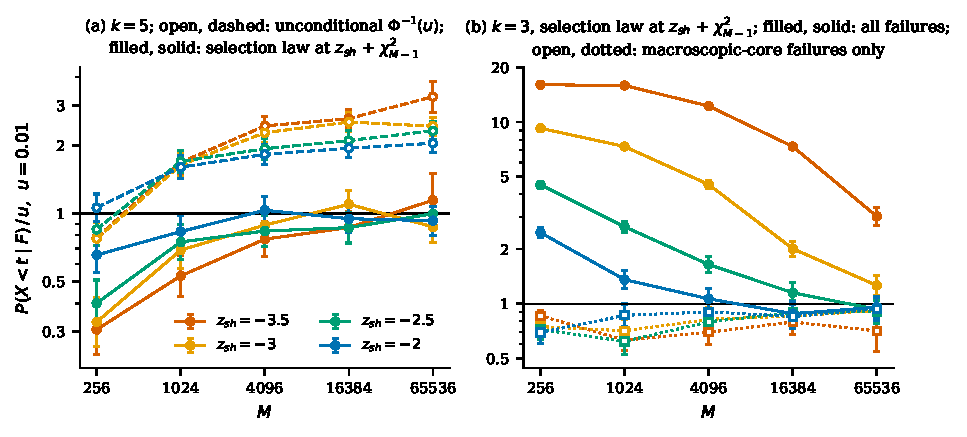
\includegraphics[width=\linewidth]{figures/fig_leftrisk.pdf}
\caption{deep-left-tail risk. (a) $k=5$, the unconditional threshold and the selection-law threshold; (b) $k=3$, all
failure samples and the macroscopic core layer.}
\label{fig:leftrisk}
\end{figure}
\subsection{The moderate-deviation conditional law}\label{app:exp-md}
\paragraph{The moderate-deviation conditional law.} In the moderate deviation regime, macroscopic failure is already a
rare event, so we use splitting to estimate its probability and conditional distribution. The splitter was first
switched to hash seeding, which fixed the correlation between the seed streams; it was then re-checked against direct
sampling, with the criteria fixed in advance: all 16 configurations and 80 comparisons satisfy $|z|\le3.5$, the
maximum $|z|$ is $2.66$, and the fraction with $|z|>2.5$ is $3.75\%$.

On this basis, GPU splitting ($k=5$, all-positive signs, macroscopic event core$>0.1d$, 27 valid configurations) gives
the difference $\Delta\mu_{\rm sh}$ between the macroscopic-layer conditional mean and the analytic prediction of the
selection law. This difference contracts as $M^{b}$, and the fitted exponents at the three depths
$z_0=-3.5,-4.5,-5.5$ are $-0.540$, $-0.553$, and $-0.525$, with all $99\%$ intervals lying within the pre-fixed range
$[-0.75,-0.25]$. Taking $z_0=-3.5$ as an example, the difference falls from $0.157$ at $M=1024$ to $0.012$ at
$M=65536$. The measured conditional variance lies between $0.98$--$1.04$, while the selection law gives $0.984$; for
$M\ge16384$ the two differ by at most $0.015$. The ratio of the macroscopic probability to the shifted-coordinate
prediction lies between $0.76$--$1.32$, and the largest deviation of the macroscopic weight is $0.067$, all satisfying
the pre-fixed criteria.

The rejection rate of the corrected selection threshold inside the macroscopic layer is the only criterion that
deviates: the pre-fixed range is $[0.7u,1.3u]$, and 20 of the 78 test units fall outside it, all on the conservative
side (ratios $0.21$--$0.69$), concentrated on the near-one-sided compositions with $M\le4096$; for $M\ge32768$ no test
unit falls outside the range. This shows that at finite size the direction of the calibration error of the macroscopic
layer is conservative.

Finally, consider the rejection rate under failure at the true $d$. The mixture rule, the envelope rule, and the
corrected selection threshold have no rejected test unit, with maximum miss$/u$ equal to $1.043$, $1.024$, and
$1.043$. As a contrast, the unconditional threshold reaches up to $3.29$ times; the asymptotic mixture rule reaches up
to $1.72$ times in the boundary region at $k=5$, and does not shrink as $M$ grows.
\subsection{Other candidate rules in the end-to-end tests}\label{app:exp-e2e-other}
The end-to-end tests of Section~\ref{sec:e2e} also include two candidate rules, both of which under-cover and are
therefore not used as implementation rules. The first is the asymptotic mixture rule of Appendix~\ref{app:axis},
namely the asymptotic form of Proposition~\ref{prop:axis}, without threshold shift or chi-square correction; its
under-coverage reaches up to 1.2 times the nominal value. The second sets the threshold by $\widehat d$ and switches
between two thresholds; among these the gz$-6$ rule reaches up to 3.24 times, occurring at $k=3$, and the switching
rules tested reach up to 3.14 times at $k\ge5$. As a contrast, the unconditional threshold reaches up to 3.1 times at
$k\ge5$.

\subsection{Finite-size location of the mean-sign-reversal layer}\label{app:exp-wm}
\paragraph{The mean-sign-reversal layer.} Figure~\ref{fig:loadaxis} examines Proposition~\ref{prop:wm} at finite
size. Panel (a) takes $k=5$ and all-same signs, and draws two layer lines, both in shifted coordinates: one is the
equal-probability layer $\Phi(z_{\rm sh})=\lambda_M$, and the other is the mean-sign-reversal layer
$s_M\eta_k\phi(z_{\rm sh})=2\lambda_M$. The reversal layer is always deeper; at $M=2^{16}$ the two layers sit at
$t=7.66$ and $t=8.29$. Between the two layers, failures mostly come from repeated edges, but the sign of the
conditional mean is still determined by the macroscopic core.

The dots in panel (b) are assembled from two parts: the macroscopic-layer probability and mean given by splitting,
and the exact mean $2/s_M$ of the repeated-edge layer. The two configurations at $M=4096$ cross the reversal layer.
For these two configurations, the repeated-edge layer is replaced by the measured values of the planted runs, and a
joint repeated bootstrap is applied to the two layers, with the following results: at $t=6.67$, $c_F\binom d2=-5.96$
with $95\%$ interval $[-6.17,-5.75]$; at $t=7.17$, $+0.48$ with interval $[+0.39,+0.57]$; the theoretical
sign-reversal point is at $t=7.15$. Small-core failures that are neither the macroscopic core nor repeated pairs can
be controlled by finite combinatorial counting, and their effect at these two points is at most $0.0022$. For
$M\ge16384$, the deepest configuration still lies before the reversal layer, with negative mean. The finite-size
offset of the macroscopic-layer mean relative to the selection law contracts roughly as $M^{-1/2}$, and after
multiplying by $s_M$ it is an $O(1)$ quantity on the original scale, so the dots in (b) lie slightly above the
theoretical curve overall.
\begin{figure}[!htbp]
\centering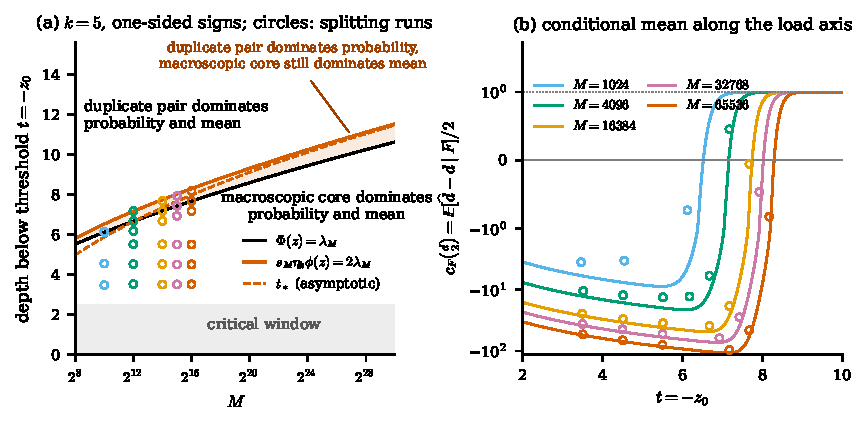
\includegraphics[width=\linewidth]{figures/fig-load-axis.pdf}
\caption{Load axis for $k=5$ and all-same signs. (a) The equal-probability layer (black) and the mean-sign-reversal
layer (orange), the dashed line is $t_*$, the dots are splitting configurations; (b) conditional mean on the original
scale, the curve is the theoretical value, the dots are the layer-wise reconstruction.}
\label{fig:loadaxis}
\end{figure}
\subsection{Supplementary checks of the analytic constants}\label{app:exp-constants}
\emph{Window width.} The measured slope $\Delta z/\Delta r$ over failure probabilities from $0.1$ to $0.9$ exceeds the
analytic value $ka_ce^{-x_c}/\sigma_k$ by $3.6\%$ ($k=5$, $M=4096$), $2.3\%$ ($k=5$, $M=16384$), and about $2\%$
($k=3$, $M=262144$), respectively, and the gap shrinks as $M$ grows. This is an independent check of $\sigma_k^2$ and
its dynamic part $\tau_k^2$.

\emph{Dynamic variance.} At $k=3$ and $M=16384$, at the moment at which the score is taken, the measured variance of
the dynamic innovation is $0.00816$, and the partial integral $\tau^2(\varepsilon_M)$ is also $0.00816$; the share held
by the initial state is consistent with $\sigma_0^2=0.01632$.

\emph{Selection strength.} At $k=6$, $M=16384$, and failure probability $0.49$, the measured slope of the Kolmogorov
distance between failure and success samples with respect to $\rho^2$ is $0.1449$, and the first-order prediction is
$0.1397$.

\subsection{Cross-check of an independent implementation}\label{app:exp-indep}
We additionally wrote a C-language sampler that shares no code with the sampler above; at the same time we recomputed
all the constants by direct numerical integration from the definition, and the results agree bit-for-bit with the
closed forms. This round did not save the seeds or the raw output, so it serves as a cross-check of an independent
implementation rather than complete reproducibility evidence. Table~\ref{tab:indep} lists the results for $M=16384$
and $r=0$. The theoretical value takes $c=\eta_k(d\rho^2-1)/(d-1)$, and $z$ takes the coordinate corresponding to the
measured failure probability. One can see that the means for $k=3$ and $k=5$ have opposite signs; the offset at
$\rho=0.6$ is about $0.36$ times that at $\rho=1$; and at $\rho=0$ the standard normal is recovered.
\begin{table}[!htbp]
\centering
\caption{Checks of the independent sampler ($M=16384$, $r=0$, 400 thousand trials per cell).}
\label{tab:indep}
\begin{tabular}{lrrrrrr}
\toprule
Configuration & $p_F$ & $\E[X\mid F]$ & theory & $\Var(X\mid F)$ & theory & KS (selection law)\\
\midrule
$k=3$, $\rho=1$ & 0.647 & $+0.2060$ & $+0.2020$ & 0.933 & 0.932 & 0.0015\\
$k=3$, $\rho=0.6$ & 0.647 & $+0.0765$ & $+0.0728$ & 0.988 & 0.991 & 0.0020\\
$k=3$, $\rho=0$ & 0.647 & $+0.0007$ & $0$ & 1.000 & 1.000 & 0.0029\\
$k=5$, $\rho=1$ & 0.659 & $-0.0744$ & $-0.0706$ & 0.990 & 0.991 & 0.0041\\
$k=5$, $\rho=0.6$ & 0.657 & $-0.0287$ & $-0.0255$ & 0.996 & 0.999 & 0.0033\\
$k=5$, $\rho=0$ & 0.658 & $+0.0018$ & $0$ & 1.000 & 1.000 & 0.0022\\
\bottomrule
\end{tabular}
\end{table}
The standard error of the mean is about $0.002$. The remaining deviation is of the same order as the threshold center
shift and the finite-size bias of the window width in Section~\ref{sec:threshold}, and shrinks as $M$ grows.
